\begin{figure}[H]
\centering
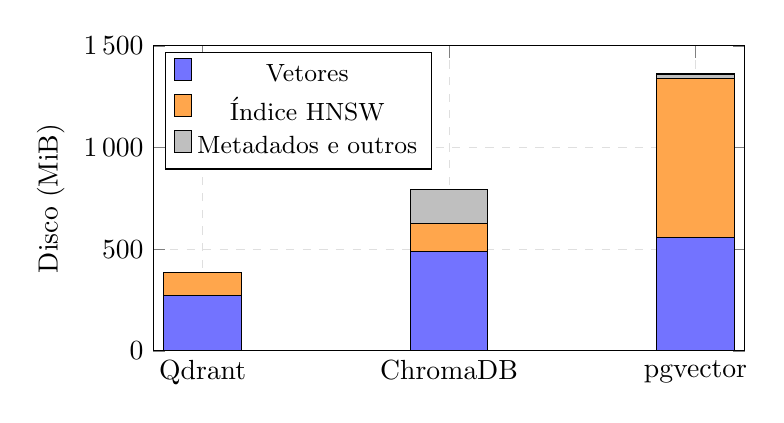
\begin{tikzpicture}
\begin{axis}[
    ybar stacked, bar width=28pt,
    width=0.75\textwidth, height=0.45\textwidth,
    ylabel={Disco (MiB)}, ymin=0, ymax=1500,
    symbolic x coords={Qdrant,ChromaDB,pgvector}, xtick=data,
    /pgf/number format/1000 sep={\,},
    legend style={at={(0.02,0.98)}, anchor=north west, font=\small},
    grid=major, grid style={dashed, gray!25}
]
\addplot[fill=blue!55] coordinates {(Qdrant,274.43) (ChromaDB,487.97) (pgvector,558.04)};
\addplot[fill=orange!70] coordinates {(Qdrant,109.94) (ChromaDB,137.74) (pgvector,781.89)};
\addplot[fill=gray!50] coordinates {(Qdrant,0.55) (ChromaDB,169.79) (pgvector,21.64)};
\legend{Vetores, Índice HNSW, Metadados e outros}
\end{axis}
\end{tikzpicture}
\caption{Decomposição do consumo de disco sob a \textbf{Métrica L2}, sem o WAL.}
\label{fig:disco_l2}
\end{figure}
